\section{FlashAttention-3: Algorithm}
\label{sec:algo}

In this section, we describe the \fat algorithm. For simplicity, we focus on the
forward pass, with the backward pass algorithm described in~\cref{sec:algo_ws_bwd}. We first indicate how to integrate warp-specialization with a circular SMEM buffer into the base algorithm of \faa. We then explain how to exploit asynchrony of WGMMA to define an overlapped GEMM-softmax 2-stage pipeline. Finally, we describe the modifications needed for FP8, both in terms of layout conformance and accuracy via block quantization and incoherent processing.

\subsection{Producer-Consumer asynchrony through warp-specialization and
  pingpong scheduling}
\label{sec:algo_ws}

\paragraph{Warp-specialization}
As with \faa, the forward pass of \fat is embarrassingly parallel in the batch size, number of heads, and query sequence length.
Thus, it will suffice to give a CTA-level view of the algorithm, which operates on a tile $\vQ_i$ of the query matrix to compute the corresponding tile $\vO_i$ of the output.
To simplify the description, we first give the warp-specialization scheme with a circular SMEM buffer that does \emph{not} have in addition the GEMM-softmax overlapping.
Let $d$ be the head dimension, $N$ the sequence length, and fix a query block size $B_r$ to divide $\vQ$ into $T_r = \lceil \frac{N}{B_r} \rceil$ blocks $\vQ_1, .., \vQ_{T_r}$.

\begin{algorithm}[H]
    \caption{\small\label{alg:flash3_wgmma_ws_only}\fat forward pass \textbf{without} intra-consumer overlapping -- CTA view}
    \begin{algorithmic}[1]
\REQUIRE Matrices $\vQ_i \in \RR^{B_r \times d}$ and $\vK, \vV \in \mathbb{R}^{N \times d}$ in HBM, key block size $B_c$ with $T_c = \lceil \frac{N}{B_c} \rceil$.
\STATE Initialize pipeline object to manage barrier synchronization with $s$-stage circular SMEM buffer.
\IF {in producer warpgroup}
\STATE Deallocate predetermined number of registers.
\STATE Issue load $\vQ_i$ from HBM to shared memory.
\STATE Upon completion, commit to notify consumer of the load of $\vQ_i$.
\FOR{$0 \le j < T_c$}
    \STATE Wait for the $(j\,\%\,s)$th stage of the buffer to be consumed.
    \STATE Issue loads of $\vK_j, \vV_j$ from HBM to shared memory at the $(j\,\%\,s)$th stage of the buffer.
    \STATE Upon completion, commit to notify consumers of the loads of $\vK_j, \vV_j$.
\ENDFOR
\ELSE
\STATE Reallocate predetermined number of registers as function of number of consumer warps.
\STATE On-chip, initialize $\vO_i = (0) \in \mathbb{R}^{B_r \times d}$ and $\ell_i, m_i = (0), (-\infty) \in \mathbb{R}^{B_r}$.
\STATE Wait for $\vQ_i$ to be loaded in shared memory.
\FOR{$0 \le j < T_c$}
\STATE Wait for $\vK_j$ to be loaded in shared memory.
\STATE Compute $\vS_i^{(j)} = \vQ_i \vK_j^T$ (SS-GEMM). Commit and wait. \label{alg:ws_only_gemm1}
\STATE Store $m_i^{\mathrm{old}} = m_i$ and compute $m_i = \max(m_i^{\mathrm{old}}, \rowmax(\vS_i^{(j)}))$. \label{code-ws:softmax_start}
\STATE Compute $\widetilde{\vP}_i^{(j)} = \exp(\vS_i^{(j)} - m_i)$ and $\ell_i = \exp(m_i^{\mathrm{old}} - m_i) \ell_i + \rowsum(\widetilde{\vP}_i^{(j)})$. \label{code-ws:softmax_end}
\STATE Wait for $\vV_j$ to be loaded in shared memory.
\STATE Compute $\vO_i = \diag(\exp(m_i^{\mathrm{old}} - m_i))^{-1} \vO_i + \widetilde{\vP}_i^{(j)} \vV_j$ (RS-GEMM). Commit and wait. \label{alg:ws_only_gemm2}
\STATE Release the $(j\,\%\,s)$th stage of the buffer for the producer.
\ENDFOR
\STATE Compute $\vO_i = \diag(\ell_i)^{-1} \vO_i$ and $L_i = m_i + \log(\ell_i)$.
\STATE Write $\vO_i$ and $L_i$ to HBM as the $i$th block of $\vO$ and $L$.
\ENDIF
\end{algorithmic}
\end{algorithm}

For our implementation of \cref{alg:flash3_wgmma_ws_only} on Hopper, we use \verb|setmaxnreg| for (de)allocations, TMA for loads of $\vQ_i$ and $\{ \vK_j, \vV_j \}_{0 \leq j < T_c}$, and WGMMA to execute the GEMMs in the consumer mainloop, with the SS or RS prefix indicating whether the first operand is sourced from shared memory or register file.
For interpreting the execution flow of \cref{alg:flash3_wgmma_ws_only}, note that issuing TMA loads does not stall on the completion of other loads due to asynchrony.
Moreover, in the producer mainloop, no waits will be issued for the first $s$ iterations as the buffer gets filled.

\paragraph{Pingpong scheduling}
The asynchronous nature of WGMMA and TMA, along with warp-specialization, opens
up the opportunity to overlap the softmax computation of one warpgroup with the GEMM of
another warpgroup.
To motivate this, notice that non-matmul operations have much lower throughput
than matmul operations on modern hardware accelerators.
As an example, the H100 SXM5 GPU has 989 TFLOPS of FP16 matmul but only 3.9
TFLOPS of special functions such as exponential\footnote{The CUDA programming
  guide specifies that 16 operations of special functions can be performed per
  streaming multiprocessor (SM) per clock cycle. We multiply 16 by 132 SMs and
  1830 MHz clock speed to get 3.9 TFLOPS of special functions.} (necessary for softmax).
For the attention forward pass in FP16 with head dimension 128, there are 512x more matmul FLOPS
compared to exponential operations, but the exponential has 256x lower
throughput, so exponential can take 50\% of the cycle compared to matmul.
The situation is even worse with FP8, where the matmul throughput doubles but
the exponential throughput stays the same.

Since the exponential is performed by a separate hardware unit (the multi-function
unit), ideally we'd want the exponential calculation to be scheduled when the
Tensor Cores are performing the matmul.
To do so, we use synchronization barriers (\texttt{bar.sync} instructions) to
force the GEMMs (GEMM1 -- $\vP \vV$ of one iteration, and GEMM0 -- $\vQ \vK^\top$
of the next iteration) of warpgroup 1 to be scheduled before the GEMMs of
warpgroup 2.
As a result, the softmax of warpgroup 1 will be scheduled while warpgroup 2 is
performing its GEMMs. Then the roles swap, with warpgroup 2 doing softmax while
warpgroup 1 doing GEMMs (hence, ``pingpong'' scheduling).
This is illustrated in~\cref{fig:pingpong_scheduling}.
Though in practice the pingpong scheduling is not as clean as depicted in the
figure, we generally find this to improve performance (e.g., from 570 TFLOPS to
620-640 TFLOPS for FP16 forward with head dimension 128 and sequence length 8192).
\begin{figure}[ht]
    \centering
    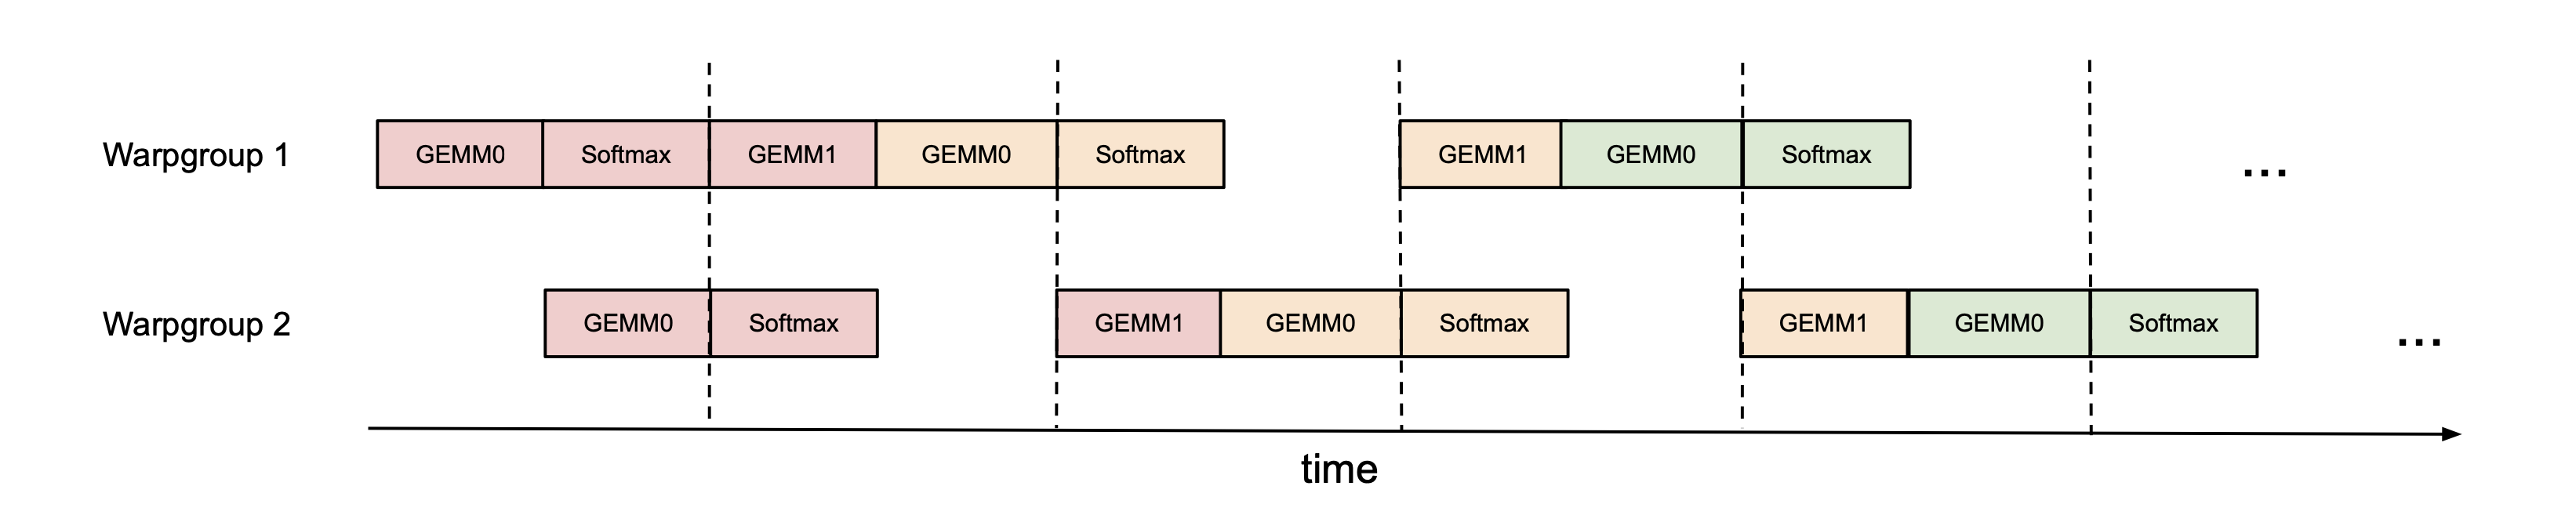
\includegraphics[width=1.0\linewidth]{figs/pingpong_pipelining.png}
    \caption{Pingpong scheduling for 2 warpgroups to overlap softmax and GEMMs: the softmax of one warpgroup
      should be scheduled when the GEMMs of another warpgroup are running. The
      same color denotes the same iteration.}
    \label{fig:pingpong_scheduling}
\end{figure}

\paragraph{Attention variants}
For multi-query attention~\citep{shazeer2019fast} and grouped query
attention~\citep{ainslie2023gqa}, we follow the approach in \faa and adjust the
tensor indexing to avoid duplicating $\vK$ and $\vV$ in HBM.

\subsection{Intra-warpgroup overlapping GEMMs and softmax}


Even within one warpgroup, we can overlap some instructions in the softmax with
some instructions in the GEMMs. We describe one technique to do so.

In the attention algorithm, operations within the inner loop (main loop) have sequential dependencies that impede parallelization within a single iteration.
For example, (local) softmax (lines \ref{code-ws:softmax_start} to \ref{code-ws:softmax_end}) relies on the output $\vS_i^{(j)}$ of the first GEMM, while the second GEMM takes its result $\widetilde{\vP}_i^{(j)}$ as an operand.
Indeed, the wait statements in lines \ref{alg:ws_only_gemm1} and \ref{alg:ws_only_gemm2} of \cref{alg:flash3_wgmma_ws_only} serialize the execution of softmax and GEMMs.
However, we can break these dependencies by pipelining across iterations through additional buffers in registers.
Pursuing this idea, we propose the following two-stage\footnote{Note that the number of stages of the overlapping scheme is bounded by, but need not equal, the number $s$ of stages in the circular SMEM buffer.} GEMM-softmax pipelining algorithm:

\begin{figure}[ht]
    \centering
    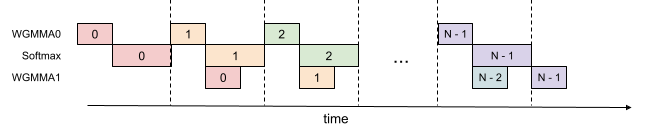
\includegraphics[width=.95\linewidth]{figs/2_stage_pipelining.png}
    \caption{2-stage WGMMA-softmax pipelining}
    \label{fig:2_stage_pipelining}
\end{figure}

\begin{algorithm}[H]
    \caption{\small\label{alg:flash3_wgmma}\fat consumer warpgroup forward pass}
    \begin{algorithmic}[1]
      \REQUIRE  Matrices $\vQ_i \in \RR^{B_r \times d}$ and $\vK, \vV \in \mathbb{R}^{N \times d}$ in HBM, key block size $B_c$ with $T_c = \lceil \frac{N}{B_c} \rceil$.
      \STATE Reallocate predetermined number of registers as function of number of consumer warps.
      \STATE On-chip, initialize $\vO_i = (0) \in \mathbb{R}^{B_r \times d}$ and $\ell_i, m_i = (0), (-\infty) \in \mathbb{R}^{B_r}$.
      \STATE Wait for $\vQ_i$ and $\vK_0$ to be loaded in shared memory.
      \STATE Compute $\vS_{\mathrm{cur}} = \vQ_i \vK_0^T$ using WGMMA. Commit and wait.
      \STATE Release the $0$th stage of the buffer for $\vK$.
      \STATE Compute $m_{i}$, $\tilde{\vP}_{\mathrm{cur}}$ and $\ell_{i}$ based on $\vS_{\mathrm{cur}}$, and rescale $\vO_i$.
      \FOR{$1 \le j < T_c - 1$}
        \STATE Wait for $\vK_j$ to be loaded in shared memory.
        \label{code:mainloop_start}
        \STATE Compute $\vS_{\mathrm{next}} = \vQ_i \vK_{j}^T$ using WGMMA. Commit but do not wait. \label{code:first_wgmma}
        \STATE Wait for $\vV_{j-1}$ to be loaded in shared memory.
        \STATE Compute $\vO_{i} = \vO_{i} + \tilde{\vP}_{\mathrm{cur}} \vV_{j-1}$ using WGMMA. Commit but do not wait. \label{code:second_wgmma}
        \STATE Wait for the WGMMA $\vQ_i \vK_{j}^T$.
        \STATE Compute $m_{i}$, $\tilde{\vP}_{\mathrm{next}}$ and $\ell_{i}$ based on $\vS_{\mathrm{next}}$. \label{code:softmax}
        \STATE Wait for the WGMMA $\tilde{\vP}_{\mathrm{cur}} \vV_{j-1}$ and then rescale $\vO_i$
        \STATE Release the $(j\,\%\,s)$th, resp. $(j-1\,\%\,s)$th stage of the buffer for $\vK$, resp. $\vV$.
        \STATE Copy $\vS_{\mathrm{next}}$ to $\vS_{\mathrm{cur}}$.
        \label{code:mainloop_end}
      \ENDFOR
      \STATE Wait for $\vV_{T_c - 1}$ to be loaded in shared memory.
      \STATE Compute
      $\vO_{i} = \vO_{i} + \tilde{\vP}_{\mathrm{last}} \vV_{T_c - 1}$ using WGMMA. Commit and wait.

      \STATE Epilogue:
      Rescale $\vO_{i}$ based on $m_{i}$.
      Compute $L_{i}$ based on $m_{i}$ and $\ell_{i}$.
      Write $\vO_{i}$ and $L_{i}$ to HBM as the $i$-th block of $\vO$ and $L$.
    \end{algorithmic}
  \end{algorithm}

  \cref{alg:flash3_wgmma} functions as a replacement for the consumer path of \cref{alg:flash3_wgmma_ws_only} to comprise the complete \fat algorithm for FP16 precision. At a high-level, we use WGMMA as a metonym for asynchronous GEMM. Within the mainloop (lines \ref{code:mainloop_start} to \ref{code:mainloop_end}), the second WGMMA operation of iteration $j$ (line \ref{code:second_wgmma}) is overlapped with softmax operations from iteration $j+1$ (line \ref{code:softmax}).

  While the pipelined structure illustrated above offers theoretical performance gains, there are several practical aspects to consider:
  \paragraph{Compiler reordering}
  The pseudocode represents an idealized execution order but the compiler (NVCC) often rearranges instructions for optimization.
  This can disrupt the carefully crafted WGMMA and non-WGMMA operation pipelining sequence, potentially leading to unexpected behavior or diminished performance gains. An analysis of the SASS code shows that the compiler generates overlapped code as expected (Section~\ref{sec:2-stage-sass}).
  \paragraph{Register pressure}
  To maintain optimal performance, register spilling should be minimized.
  However, the 2-stage pipeline requires additional registers to store intermediate results and maintain context between stages.
  Specifically, an extra $\vS_{\mathrm{next}}$ must be kept in registers, leading to extra register usage of size $B_r \times B_c \times \text{sizeof}(\text{float})$ per threadblock.
  This increased register demand may conflict with using larger block sizes (another common optimization), which is also register-hungry.
  In practice, trade-offs should be made based on profiling results.
  \paragraph{3-stage pipelining} Extending the 2-stage algorithm described above, we propose a 3-stage variant
  that would further overlap the second WGMMA with softmax.
  While this approach offers the potential for even higher Tensor Core utilization,
  it requires even more registers due to an additional stage in the pipeline,
  making the trade-off between tile size and pipeline depth more difficult to balance.
  A detailed description of the 3-stage algorithm and its evaluation results can be found in ~\cref{sec:3-stage}.

\subsection{Low-precision with FP8}
\label{sec:algofp8}

\begin{figure} %
\centering
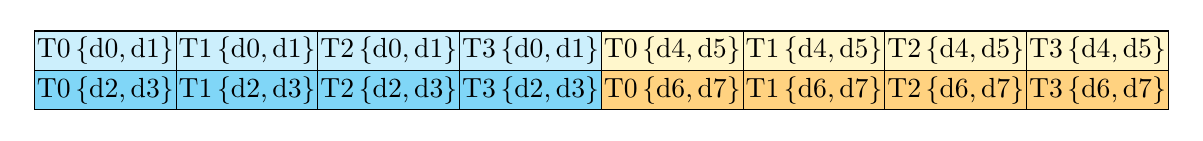
\begin{tikzpicture}
\definecolor{mygold}{RGB}{255, 215, 0} %
\definecolor{warmcolor}{RGB}{255, 165, 0} %
\def\r{.9}
\def\h{-.5}
\foreach \y in {0,2} {
  \ifnum\y=0
    \def\mycolor{cyan!20}
  \else
    \def\mycolor{mygold!20}
  \fi
  \foreach \x in {0,2} {
    \draw[fill=\mycolor] (4*\y*\r+\x*\r,0) rectangle ++(2*\r,.5);
    \draw[fill=\mycolor] (4*\r+4*\y*\r+\x*\r,0) rectangle ++(2*\r,.5);
  }
}
\foreach \y in {0,2} {
  \ifnum\y=0
    \def\mycolor{cyan!50}
  \else
    \def\mycolor{warmcolor!50}
  \fi
  \foreach \x in {0,2} {
    \draw[fill=\mycolor] (4*\y*\r+\x*\r,\h) rectangle ++(2*\r,.5);
    \draw[fill=\mycolor] (4*\r+4*\y*\r+\x*\r,\h) rectangle ++(2*\r,.5);
  }
}

\foreach \y in {0,2} {
  \foreach \x in {0} {
    \ifnum\y=0
      \node at (4*\y*\r+\x*\r + \r, 0.25) {T0\,\{d0,\,d1\}};
    \else
      \node at (4*\y*\r+\x*\r + \r, 0.25) {T0\,\{d4,\,d5\}};
    \fi
  }
  \foreach \x in {2} {
    \ifnum\y=0
      \node at (4*\y*\r+\x*\r + \r, 0.25) {T1\,\{d0,\,d1\}};
    \else
      \node at (4*\y*\r+\x*\r + \r, 0.25) {T1\,\{d4,\,d5\}};
    \fi
  }
}
\foreach \y in {1,3} {
  \foreach \x in {0} {
  \ifnum\y=1
    \node at (4*\y*\r+\x*\r + \r, 0.25) {T2\,\{d0,\,d1\}};
  \else
    \node at (4*\y*\r+\x*\r + \r, 0.25) {T2\,\{d4,\,d5\}};
  \fi
  }
  \foreach \x in {2} {
  \ifnum\y=1
    \node at (4*\y*\r+\x*\r + \r, 0.25) {T3\,\{d0,\,d1\}};
  \else
    \node at (4*\y*\r+\x*\r + \r, 0.25) {T3\,\{d4,\,d5\}};
  \fi
  }
}

\foreach \y in {0,2} {
    \foreach \x in {0} {
      \ifnum\y=0
        \node at (4*\y*\r+\x*\r + \r, 0.25+\h) {T0\,\{d2,\,d3\}};
      \else
        \node at (4*\y*\r+\x*\r + \r, 0.25+\h) {T0\,\{d6,\,d7\}};
      \fi
    }
    \foreach \x in {2} {
      \ifnum\y=0
        \node at (4*\y*\r+\x*\r + \r, 0.25+\h) {T1\,\{d2,\,d3\}};
      \else
        \node at (4*\y*\r+\x*\r + \r, 0.25+\h) {T1\,\{d6,\,d7\}};
      \fi
    }
  }

\foreach \y in {1,3} {
  \foreach \x in {0} {
  \ifnum\y=1
    \node at (4*\y*\r+\x*\r + \r, 0.25+\h) {T2\,\{d2,\,d3\}};
  \else
    \node at (4*\y*\r+\x*\r + \r, 0.25+\h) {T2\,\{d6,\,d7\}};
  \fi
  }
  \foreach \x in {2} {
  \ifnum\y=1
    \node at (4*\y*\r+\x*\r + \r, 0.25+\h) {T3\,\{d2,\,d3\}};
  \else
    \node at (4*\y*\r+\x*\r + \r, 0.25+\h) {T3\,\{d6,\,d7\}};
  \fi
  }
}
\end{tikzpicture}
\caption{FP32 accumulator register WGMMA layout -- rows 0 and 8, threads 0-3, entries 0-7.}
\label{fig:rmem_accum}
\end{figure}

\begin{figure}
\centering
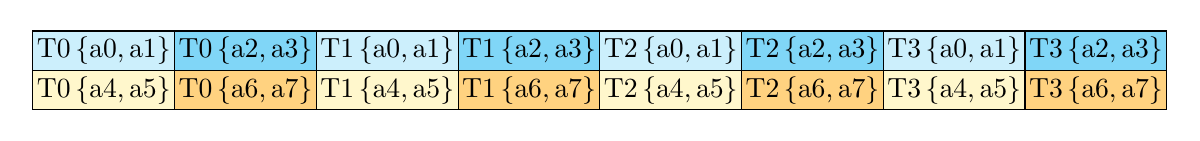
\begin{tikzpicture}
\definecolor{mygold}{RGB}{255, 215, 0} %
\definecolor{warmcolor}{RGB}{255, 165, 0} %
\def\r{.9}
\def\h{-.5}

\foreach \y in {0,...,3} {
  \foreach \x in {0,2} {
    \ifnum\x=0
      \def\mycolor{cyan!20}
    \else
      \def\mycolor{cyan!50}
    \fi
    \draw[fill=\mycolor] (4*\y*\r+\x*\r,0) rectangle ++(2*\r,.5);
  }
}
\foreach \y in {0,...,3} {
  \foreach \x in {0,2} {
    \ifnum\x=0
      \def\mycolor{mygold!20}
    \else
      \def\mycolor{warmcolor!50}
    \fi
    \draw[fill=\mycolor] (4*\y*\r+\x*\r,\h) rectangle ++(2*\r,.5);
  }
}
\foreach \y in {0,...,3} {
    \foreach \x in {0,2} {
      \ifnum\x=0
        \node at (4*\y*\r+\x*\r + \r, 0.25) {T\y\,\{a0,\,a1\}};
      \else
        \node at (4*\y*\r+\x*\r + \r, 0.25) {T\y\,\{a2,\,a3\}};
      \fi
    }
}
\foreach \y in {0,...,3} {
    \foreach \x in {0,2} {
      \ifnum\x=0
        \node at (4*\y*\r+\x*\r + \r, 0.25+\h) {T\y\,\{a4,\,a5\}};
      \else
        \node at (4*\y*\r+\x*\r + \r, 0.25+\h) {T\y\,\{a6,\,a7\}};
      \fi
    }
}
\end{tikzpicture}
\caption{FP8 operand A register WGMMA layout -- rows 0 and 8, threads 0-3, entries 0-7.}
\label{fig:rmem_operand}
\end{figure}

\textbf{Efficiency: layout transformations.}
Computing the forward pass of \fat in FP8 precision poses additional challenges not encountered for FP16 in terms of layout conformance.

First, we note that the input tensors $\vQ$, $\vK$, and $\vV$
are typically given as contiguous in the head dimension,
while to satisfy the k-major constraint on FP8 WGMMA for the second GEMM we need $\vV$,
or rather the tiles of $\vV$ loaded into SMEM, to be contiguous in the sequence length dimension.
Since the TMA load itself cannot change the contiguous dimension, we then need to either
(1) transpose $\vV$ in GMEM as a pre-processing step, or
(2) do an in-kernel transpose of tiles of $\vV$ after loading them into SMEM.
To implement option (1), we can either
(1a) fuse the transpose to the epilogue of a preceding step such as the rotary embedding, or
(1b) call a standalone pre-processing transpose
kernel\footnote{An optimized transpose kernel will achieve speed near the bandwidth of the device~\citep{colfax_cutlass_transpose_2024}.}
to exchange the strides of the sequence length and head dimensions.
However, (1a) is difficult to integrate into a standard library,
and (1b) is too wasteful in a memory-bound situation such as inference.

Instead, for FP8 \fat we opt for option (2).
For the in-kernel transpose, we take advantage of the LDSM (\verb|ldmatrix|)
and STSM (\verb|stmatrix|) instructions,
which involve a warp of threads collectively loading SMEM to RMEM
and storing RMEM to SMEM at a granularity of 128 bytes.\footnote{In the PTX documentation, LDSM/STSM are described as copying $8 \times 8$ matrices with 16-bit entries \cite[\S 9.7.13.4.15-16]{ptx},
but we can pack 8-bit entries two at a time to use LDSM/STSM in the context of FP8 precision.
However, the transpose versions of LDSM/STSM cannot split packed 8-bit entries,
which necessitates certain register movements in between LDSM and STSM to actually perform a tile-wise transpose; we omit the details.}
The LDSM/STSM instructions are both register efficient,
allowing us to execute them in the producer warpgroup,
and capable of transposing layouts when doing memory copy.
Moreover, after the first iteration we can arrange
for the transpose of the next $\vV$ tile
to be executed in the shadow of the two WGMMAs
that involve the preceding $\vV$ and current $\vK$ tile.

Second, we observe that unlike with FP16,
the memory layout of the FP32 accumulator of an FP8 WGMMA is different
from that assumed for its operand A when held in registers.
We depict fragments of these two layouts in \cref{fig:rmem_accum} and \cref{fig:rmem_operand},
where the entries are held in registers per thread in the listed order.
By using byte permute instructions,
we can then transform the first WGMMA's accumulator into a format suitable for the second WGMMA,
and compatibly with the layout of the $\vV$ tile produced by the in-kernel transpose. Specifically, with reference to \cref{fig:rmem_accum}, we change the order in sequence to
$$\{ \verb|d0 d1 d4 d5 d2 d3 d6 d7| \},$$
and this register permutation is then replicated over every 8 bytes. In terms of the logical shape of the $\vP$ tile, this manuever permutes its columns (e.g., columns $0189$ now become the first four columns). For WGMMA to then compute the correct output tile, we can correspondingly arrange for the in-kernel transpose to write out a matching row permutation of the $\vV$ tile.\footnote{This additional freedom afforded by doing the in-kernel transpose eliminates having to use shuffle instructions to change register ownership across threads, which we previously described in~\citep{colfax_fp8_flashattention_2024}.}






\textbf{Accuracy: block quantization and incoherent processing.}
With FP8 (e4m3) format, one only uses 3 bits to store the mantissa and 4 bits
for the exponent.
This results in higher numerical error than FP16/BF16.
Moreover, large models typically have outlier values~\citep{dettmers2208llm,
  sun2024massive} that are much larger in magnitude than most other values,
making quantization difficult.
One typically use per-tensor scaling~\citep{micikevicius2022fp8} by keeping one scalar per tensor (e.g., one
for $\vQ$, for $\vK$, and for $\vV$).
To reduce the numerical error of attention in FP8, we employ two techniques:
\iftoggle{arxiv}{
\begin{enumerate}
}{
\begin{enumerate}[itemsep=0pt,topsep=0pt,leftmargin=*]
}
\item \textbf{Block quantization}: we keep one scalar per block, so that
 for each of $\vQ$, $\vK$, $\vV$ we split the tensor into blocks of
  size $B_r \times d$ or $B_c \times d$ and quantize them separately.
  This quantization can be fused with an operation right before attention (e.g.,
  rotary embedding) with no additional slow down (since rotary embedding is
  memory-bandwidth bound).
  As the \fat algorithm naturally operates on blocks, we can scale each block of
  $\vS$ to account for this block quantization at no computation cost.
\item \textbf{Incoherent processing}: to even out outliers, we multiply
  $\vQ$ and $\vK$ with a random orthogonal matrix $\vM$ before quantizing to
  FP8. Since $\vM$ is orthogonal, $\vM \vM^\top = I$ and so $(\vQ \vM) (\vK
  \vM)^\top = \vQ \vK^\top$, i.e., multiplying both $\vQ$ and $\vK$ with
  $\vM$ does not change the attention output.
  This serves to ``spread out'' the outliers since each entry of $\vQ \vM$
  or $\vK \vM$ is a random sum of entries of $\vQ$ or $\vK$, thus reducing
  quantization error.
  In practice, we follow \citet{chee2024quip} and~\citet{tseng2024quip} and choose $\vM$ to be the product of random diagonal matrices of $\pm
  1$ and a Hadamard matrix, which can be multiplied in $O(d \log d)$ instead of
  $O(d^2)$, and can also be fused with the rotary embedding at no extra computation cost.
\end{enumerate}
We validate that these two techniques reduces numerical error by up to 2.6$\times$ in \cref{sec:numerical_error}.
